\documentclass{article}
\usepackage[utf8]{inputenc}
\usepackage{authblk}
\usepackage{graphicx}
\usepackage{amsmath}
\usepackage{ctable}
\usepackage{tabu}
\usepackage{hyperref}
\usepackage{svg}
\usepackage{gensymb}
\usepackage[
backend=biber,
style=numeric,
]{biblatex}
\usepackage{tabularx} % in the preamble

\addbibresource{bib.bib}
\graphicspath{{GFX/}}

\title{MSR Xenon Analysis: Review and Decomposition}
\author[1]{Terry J. Price\thanks{Terry.Price@uoit.net}}
\author[1]{Ondrej Chvala\thanks{OChvala@utk.edu}}
\affil[1]{University of Ontario Institute of Technology}
\affil[2]{University of Tennessee Knoxville}
\date{July 2018}

\begin{document}

\maketitle


\section{Introduction}
\subsection{Overview}
The behavior of xenon is of principal importance in the prediction and description of nuclear reactor behavior.  This document discusses the relevant features, governing equations, and constitutive formula involved in the analysis of xenon in a Molten Salt Reactor (MSR).  This document is designed to be used in conjunction with the Oak Ridge reports ORNL-4069, ORNL-TM-3464, and the appendix of ORNL-TM-4541. \cite{ORNL4069} \cite{ORNLTM3464} \cite[p. 170]{Robertson1971}

A MSR uses circulating alkali fluoride fuel salt melt as both a fuel matrix and a working fluid. MSR development started in the 1950s at the Oak Ridge National Laboratory (ORNL) in the United States.  This effort reached apogee with the design, development, and subsequent operation of the Molten Salt Reactor Experiment (MSRE) in the 1960s.  The MSR program at ORNL resulted in several conceptual designs of large MSR power systems,  the final one being the Denatured Molten Salt Reactor (DMSR) published in the 1980s.  Details about the history of the MSR program at ORNL are documented by MacPherson and Dolan \cite{MacPherson1985} \cite[p. 2]{Dolan2017} Renewed interest of MSRs is coincident with their inclusion among the Generation IV concepts (GenIV), see Serp. \cite{Serp2014}

For our purposes, let us undergo a brief familiarization with the structural and process components of a simple single-fluid MSR. The description hereafter is not specific to any particular MSR concept. The description stated hereafter is a Technological Level description using the terminology of Lorenz; that is, it is a description of the system at level of components, which are given as \textit{black-boxes}.\cite{Lorenz1996}
The key components of an MSR are shown in Figure \ref{MSRLoop}.
\label{MSRLoop}
\begin{figure}[ht]
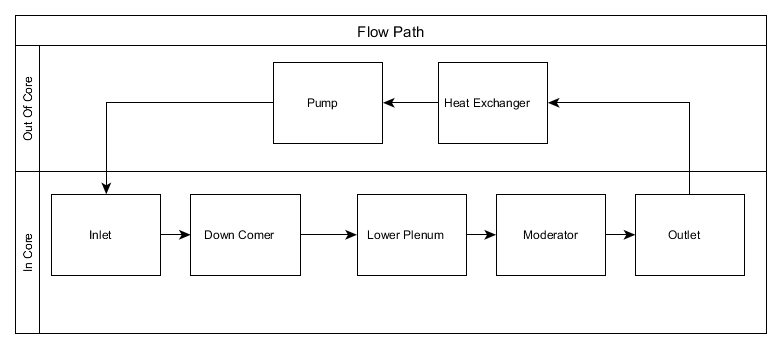
\includegraphics[width=\textwidth,height=\textheight,keepaspectratio]{MSRLoop.png} 
\caption{MSR Flow Path}
\end{figure}

Fuel enters the reactor vessel through the inlet and moves down to the lower plenum via the down comer.  Once in the lower plenum, the fuel salt intramixes and travels up the fuel channels which have been cut into graphite stringers.  The graphite stringers constitute the moderator. When within the moderating region, the fuel undergoes fission and heat is generated. Once the fuel salt has passed through the fuel channels, it leaves the reactor through the outlet and enters the heat exchanger where it deposits its heat content. The fuel salt then leaves the heat exchanger and enters the fuel pump where momentum is imparted into it from the impeller. The fuel salt then leaves the pump and enters the inlet where the cycle is repeated. Pressure is maintained in reactor vessel via the cover gas in the upper plenum.  Cover gas is injected into the upper plenum via the cover gas inlet and removed via the cover gas outlet.  The entire primary circuit can be divided into in-core and out-of-core volumes. The flow paths through these volumes is illustrated below. The primary circuit will likely also contain additional components, which have not been depicted, including a dedicated gas stripper, equipment to sample salt, adjust chemistry, refuel the reactor, etc.

The migratory behavior of xenon in molten salt is qualitatively different than that in solid fuel.  When the fuel is solid the migration of xenon is of secondary importance to the analysis of xenon behavior. In an MSR, the xenon circulates with the fuel salt, and undergoes a number of mass transfer processes in the various regions of the reactor. This includes a possibility to remove xenon (and other fission gases) off the fuel, which is a unique capability of molten fuel.   After its production via nuclear fission or the decay of iodine, the xenon moves about the reactor dissolved in the salt, in the circulating gaseous voids (bubbles), diffusing into the moderating graphite, or leaving the core to cover gas or through offgasing equipment.  The source, sink and migration processes in MSR xenon theory are summarized in Table \ref{termTable}.
\begin{table}[ht]
\begin{tabularx}{\linewidth}{ |X|X|X| }
  \hline
 \textbf{Source Terms} & \textbf{Sink Terms} & \textbf{Migration Terms} \\
  \hline 
  Fission Production  & Radioactive Decay  & Mass Transfer to Circulating Voids   \\
  \hline
  Production From Progenitors & Burn Out & Removal via Cover Gas Outlet Line \\
   \hline
    & Removal via Cover Gas Outlet Line & Mass Transfer to Cover Gas \\
   \hline
\end{tabularx}
\caption{Terms in MSR Xenon Analysis }
\label{termTable}
\end{table}






Figure \ref{XeBlocks} shows a qualitative description of processes in MSR xenon theory. $^{135}Xe$  originates from either fission or the $^{135}Xe$  progenitors, $^{135}I$  and $^{135}Te$ . The aforementioned isotopes, henceforth described as \textit{poison species},  are all fission products and are produced in nuclear fission. $^{135}Te$ transmutes into  $^{135}I$ which transmutes into  $^{135}Xe$.$^{135}Xe$  transmutes into $^{135}Cs$. All the previously mentioned decay processes are facilitated through beta minus decay.  The poison species are all formed inside of the fuel salt.  The  $^{135}Te$ and  $^{135}I$ remain in solution in the fuel salt, whereas the  $^{135}Xe$ is able to migrate from the fuel salt to the cover-gas, circulating voids (bubbles), and cover-gas due to its noble and gaseous nature. There may also be mass transfer directly from bubbles to the graphite.  The absorption cross sections of  $^{135}Te$ and  $^{135}I$ are assumed to be negligible.  In addition to burn-up and radioactive decay,  $^{135}Xe$ may be removed from the system from removal of the cover-gas.  There is a distinction in terminology between diffusive off-gassing and mechanical sparging.  In off-gassing, diffusion drives dissolved gas past an interface whereas sparging refers to a mechanical gas removal process. An example of sparging is the xenon spray-ring in the Molten Salt Reactor Experiment (described later).  The ORNL literature uses the term stripping occasionally in place of sparging.

\begin{figure}[ht]
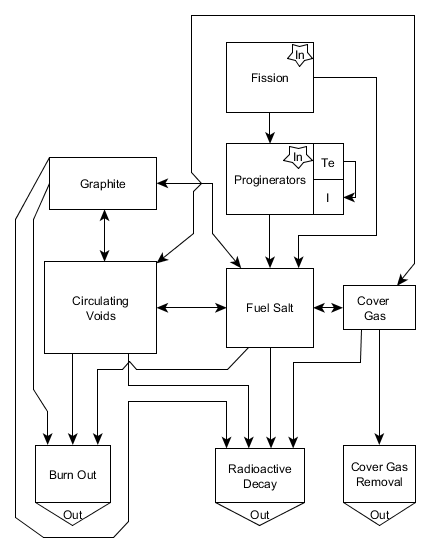
\includegraphics[width=\textwidth,height=\textheight,keepaspectratio]{XeBlocks.png} 
\caption{Xenon Mass Transfer Pathways}
\label{XeBlocks}
\end{figure}
\subsection{Xenon In Historical MSRs}
There were three experimental MSRs that were built and operated: the Aircraft Reactor Experiment (ARE); the Pratt and Whitney Aircraft Reactor-1 (PWAR-1); and, the Molten Salt Reactor Experiment (MSRE).

The Aircraft Reactor Experiment (ARE) was designed to demonstrate basic features in an effort to develop a nuclear propulsion source on an aircraft. \footnote{A reactor referred to as the \textit{Fused Salt Reactor Experiment} (FSRE) is described in the report by Ergen.\cite{Egen1957}  The description of this reactor is similar to that of the ARE.  We posit that the FSRE is the same reactor as the ARE.}  ARE used a NaF-ZrF4-UF4 fuel salt, a beryllium oxide moderator, and outlet temperature of 1133 K.\cite[p. 62]{OSullivan2015} The ARE operated for 100 MW-hours over the course of nine days in 1954. [ibid] Bettis reports that the positive temperature coefficient of reactivity related to xenon poisoning in solid fuel reactors was considered to be significant enough to warrant abandoning them in design considerations for the ARE project.\cite{Bettis1957} The ARE used a xenon removal system built into the fuel-pumps. The xenon removal system was comprised of a mixing chamber in which the fuel salt was sprayed through a helium atmosphere on to the mixing chamber wall.  The result was a foam/salt mixture with a high gas-interface surface area.  The large surface area facilitates the transfer the gaseous fission products from the salt to the gas. The foam/salt mixture was then pumped into an expansion volume, where the helium and gaseous products therein were removed via an off-gas system.\cite[pp. 31-32]{Fraas1956} An experiment performed on the ARE, named Experiment H-11,   showed that no more than 5\% of the xenon in the produced by the reactor remained in the fuel salt.\cite[p. 67]{ORNL1845}  This poison fraction was determined by finding the predicted reactivity lost from xenon poisoning without any xenon removal, and comparing it to measured amount of xenon poisoning. 

The Pratt and Whitney Aircraft Reactor (PWAR-1) was zero-power test bed with a beryllium moderator and reflector. \cite[p. 286]{Dolan2017} Critical, zero-power experiments with external heating were performed on the reactor in 1957.  \cite[p. 2]{ORNL2536} No information on xenon behavior in the PWAR-1 was found. 

The Molten Salt Reactor Experiment (MSRE) was an 8 MWth graphite moderated MSR built and operated in the 1960s.\cite[p. 376]{MacPherson1985}  The MSRE underwent two distinct operational phases, one with a U-235 based fuel salt, starting in 1965, and another with a U-233 based fuel salt, starting in 1968.\cite[p. 6]{Forsberg2006} The two major reports that detail xenon behavior in the MSRE were ORNL-4069 and ORNL-TM-3464.\cite{ORNL4069,ORNLTM3464}

Two models were generated in ORNL-4069, one with, and another without bubbles included. The experience leading to the decision to include bubbles in the model is described in ORNL-TM-1796. \cite[p. 14]{ORNLTM1796} Both of these models included considerations for the xenon stripper,  absorption into graphite, and xenon progenitors.  The reactor was subdivided into 72 annular regions, and the xenon poisoning was formulated for each region.  The per-region poisoning was weighted by the adjoint flux, and the poisoning for the entire reactor was found by summing across all the regions.  Sensitivity analyses were performed with both models. ORNL-4069 (published in 1967) indicated that at higher void fractions, the majority of the xenon would be found in the circulating bubbles rather than the graphite or fuel salt. \cite[p. 56]{ORNL4069} This finding is preceded by a report in ORNL-4037, wherein Prince et al. state,

\begin{quote}
"This plot [showing xenon distribution in graphite, fuel-salt, and bubbles as a function of circulating void fraction] shows show circulating bubbles work to decrease the loss of reactivty to $^{135}Xe$ .  As the void fraction is increased, most of the dissolved xenon migrates to the bubbles, dropping the dissolved xenon concentration greatly. The concentration potential [driving force] necessary for $^{135}Xe$  to migrate to the graphite is reduced accordingly." \cite[p. 15]{ORNL4037}
\end{quote}

This is a new development, for in 1961, the analysis by Miller, which ignored circulating bubbles, showed that given his assumptions, the majority of xenon was found in the graphite. \cite[p. 7]{Miller1961} The claim in ORNL-4069, that bubbles may contain significantly more xenon than the fuel salt, was corroborated, in ORNL-TM-3027 (published 1970 by Engel et al.) which states that a few bubbles dispersed in the fuel salt can contain far more xenon than all of the salt.\cite[p. 47]{ORNLTM3027} ORNL-4069 concludes with the following xenon-related conclusions\cite[p. 58]{ORNL4069}:

\begin{enumerate}
  \item The presence or lack of bubbles has a significant impact on the outcome of the model.  When bubbles were included in the model, the xenon poison fraction could be made to agree with preliminary observed xenon poison fractions.
  \item Many assumptions including the volatization of iodine were made in the model, and the model ought not be considered final.
  \item $^{135}Xe$ poisoning shows an insensitivity to the void fraction and diffusion coefficient of the graphite. 
\end{enumerate}

The other major report detailing xenon in the MSRE was ORNL-TM-3464, written in 1971. \cite{ORNLTM3464} The report provides a description of processes affecting $^{135}Xe$ behavior in the MSRE; predictions about MSRE xenon behavior; observations of xenon behavior during the MSRE operation; an analysis of xenon within the MSRE cover-gas; details the generation of a model that describes MSRE xenon behavior; and, discusses the results of this model. 

Two separate xenon models were developed in ORNL-TM-3464, one for soluble, and another for insoluble cover-gas.  The model that assumed a soluble cover-gas used a separate, coupled cover-gas model, whereas the model that assumed an insoluble cover-gas used an integrated cover-gas model.  The structure of the xenon model was as follows: regions contained sub-regions, which contained nodes.  One isotopic species concentration was associated with each node. The fuel-loop was treated in four regions, each treated as a well-stirred tank.  The regions were the pump-bowl piping and heat exchanger,  reactor core, and piping to the pump bowl
.  The piping and heat exchanger was further divided into liquid and gas-bubble sub-regions.  The reactor core was subdivided into a liquid, gas-bubble sub-regions, and six graphite sub-regions.  The piping to the pump bowl was identical to the piping and heat exchanger sub-region in that it contained both liquid and gas-bubble sub-regions.  Finally, the pump bowl had sub-regions for the gas-space, old bubbles, and liquid.  Each sub-region had nodes for $^{135}I$, $^{135}Xe$, and $^{135m}Xe$ where appropriate. The graphite within the core was subdivided into four radial regions with mass-transfer between the regions accounted for by diffusion.  Subdivision was in the radial direction, however, unlike the xenon model in ORNL-4069, no facility was made for breakdown in the axial direction. Each radial region had appropriate regional flux and nuclear importance incorporated into its behavior.  Each of the nodes had a material balance equation written on it in the form of a system of first-order linear differential equations. This system was then solved for both the steady-state solution vector as well as for the transient behavior.

ORNL-TM-3464 concludes the following\cite[96]{ORNLTM3464}:
\begin{enumerate}
    \item The totality of xenon behavior for MSRs had not been accurately predicted by prior analyses
    \item Subsequent analyses have been partially successful in describing xenon behavior, but there continues to be areas of uncertainty
    \item There was a considerable difference in xenon behavior depending on if Helium or Argon cover gas was used.
    \item Attempts at reactor behavior description required liquid/gas mass transfer coefficients, and stripping efficiencies substantially different than the predicted values.
    \item Description of xenon behavior required considerations for mass transfer from the circulating voids to the graphite. 
    \item The circulating void to graphite behavior was a function of both circulating void size and fraction.
\end{enumerate}
Finally, ORNL-TM-3464 posses a set of five research questions. The authors of ORNL-TM-3464 believe the answer to these research question will lead to increased accuracy in the modeling of MSR xenon behavior.  No detailed attempts at answering these questions have been found, but some ...TODO

circ voidds/ bubbles fraction, seze.
xenon behavior...
\subsection{Properties of Relevant Isotopes and Fuel Salt}
\label{sec:fuelSaltProperties}
There are three isotopes we are chiefly concerned with, $^{135}Te$, $^{135}I$, and $^{135}Xe$.  Collectively, we shall refer to these isotopes as the \textit{poison isotopes} Some analyses, such as that in ORNL-TM-1070 ignore Tellerium.  The effects of $^{135m}Xe$ have also been investigated in ORNL-TM-3464 and by Eades.\cite{ORNLTM3464,Eades16}  

The poison species progress down the decay chain through nuclear decay. The $^{135}Te \rightarrow ^{135}I \rightarrow ^{135}Xe$ chain with a $^{135m}Xe$ branch is depicted in figure \ref{fig:XeDecay}. \begin{figure}[ht]
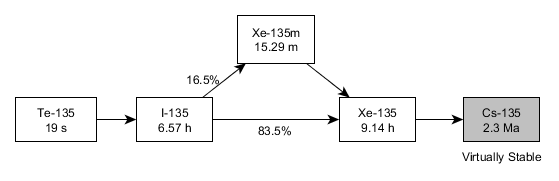
\includegraphics[width=\textwidth,height=\textheight,keepaspectratio]{XeDecay.png} 
\caption{Xe Decay Chain}
\label{fig:XeDecay}
\end{figure} Te-135 decays into I-135 through beta minus decay with a 19 s half-life. \cite[p. 56]{Baum2010}  Iodine then undergoes beta minus decay and transmutes into either Xe-135 or the meta-stable form, Xe-135m  6.57 h half-life. [ibid.] Any Xe-135m formed de-excites into Xe-135 through gamma emanation with a 15.3 m half-life. \cite[p. 298]{Eades16} Xe-135 finally transmutes into Cs-135 with a half-life of 9.14h.\cite[p. 56]{Baum2010} The Cs-135 is virtually stable with its 2.3 My half-life. [ibid]  All of these poison isotopes are both produced directly from fission, as the product of other nuclear reactions, and from radioactive decay.

The thermal neutron absorption cross section for xenon-135 is 2.6 Mb. \cite[p. 54-9]{Mughab12P1} The neutron absorption cross section for Xe-135 averaged over the MSRE neutron spectrum is 1.18 Mb\footnote{This claim is based on a personal communication between the authors of ORNL-4069 and B.E. Prince.  No details as to how this value was arrived at are given.}.\cite[p. 42]{ORNL4069} [ The xenon model in ORNL-4069 did not include any considerations of Xe-135m; however, the xenon model in ORNL-TM-3464 did. The ORNL-TM-3464 xenon model did not include any consideration for neutron absorption in Xe-135m since the cross-section was was unknown at the time. \cite[p. 3]{ORNLTM3464}  Since then, Eades, who reported the Xe-135m thermal neutron absorption cross-section is 10 Mb, has investigated its effect on MSRs.\cite{Eades16}

The thermophysical properties of molten salt influence the behavior of xenon in an MSR.  Yoder warns that the accuracy of heat transfer correlations in molten salt systems are limited by the accuracy of the thermophysical properties.\cite{Yoder2014} By extension, the accuracy of mass-transfer correlations, through heat/mass transfer analogies, are limited by the accuracy of thermophysical properties.  Some sources of thermophysical data are for use in modeling efforts are given by Cantor, Sohal, and Janz. \cite{ORNLTM2316,Sohal2010,Janz2013} In the work by Cantor, fuel salt F4 is closest in composition to enriched MSRE fuel salt as given in ORNL-TM-0728.  The uranium enrichment of fuel-salt F4 was not found. Nevertheless, given the 1.3\% difference in mass between U-235 and U-238 is about 1.3\%, the difference in thermophysical properties between enriched an unenriched fuel salt can be assumed to be negligible.  In addition to these data, Grimes, Blander, and Watson give information on solubility limits and Henry’s constants for xenon and other noble gases.\cite{Grimes1958, Blander1959, Watson1962} Note the temperature and pressure dependence of Henry’s constants and xenon solubility limits. 

\subsection{Xenon Production and Evolution}

Xenon and its progenitors are produced as fission products.  It is assumed that neutron induced fission is the only significant source of fission in an MSR, and fission pathways such as photofission or muon induced fission from extraterrestrial radiation are insubstantial.  The fission production rate is given by,

\begin{equation}
    \dot{N} = \int \int_{RC} \gamma_i \Sigma_f(E,\vec{x}) \phi(E,\vec{x}) dV dE
\end{equation}

where the volume of integration is the reactor core volume (i.e., not the external loop).  The fission yield, $\gamma_i$,  gives a probability of producing a particular fission nuclide and depends on the actinide in which the fission occurs, and the incident neutron energy.  The Japanese Atomic Energy Agency maintains a user friendly database of fission product yields (JENDL). \cite{JENDLFP}  A table detailing the fission product yields of xenon and its progenitors of some actinides found in nuclear fuel is shown in table \ref{tbl_fp}.
\begin{table}[h]
\begin{tabularx}{\linewidth}{ |X|X|X|X| }
  \hline
  & \textbf{Xe-135} & \textbf{I-135} & \textbf{Te-135} \\
  \hline 
  U-235  & 0.257  & 2.935  & 3.225 \\
  \hline
  Pu-239 & 1.066 & 4.286 & 2.192 \\
   \hline
   Pu-241 & 0.227  &  3.001 & 3.729  \\
   \hline
\end{tabularx}
\caption{Fission product yields (in \% of fissions resulting in a given product) of poison species for three different actinides. \cite{JENDLFP}}
\label{tbl_fp}
\end{table}
Two observations can be made from this table.  First, Xe-135 is consistently has the smallest fission product compared to I-135 and Te-135.  Therefore  xenon poisoning predominately arises from the progenitor inventory rather than directly from fission. Second since the nuclear fuel changes actinide composition with burn-up, and the fission yield is a function of actinide it occurs in, it follows that the xenon poisoning will also change.

The time evolution of xenon in the system, without any mass transfer, can be described by set of three coupled ordinary differential equations,

\begin{subequations}
\begin{align}
\dot{N}_{Xe} &=  \gamma_{Xe} \Sigma_f \phi V_{RC} + \lambda_I N_I -\lambda_{Xe} N_{Xe} - \Sigma_a^{Xe} \phi V_{RC}, \\
\dot{N}_I &=\gamma_{I} \Sigma_f \phi V_{RC} - \lambda_I N_I + \lambda_{Te} N_{Te}, \\
\dot{N}_{Te} &= \gamma_{Te} \Sigma_f \phi V_{RC} - \lambda_{Te} N_{Te} .
\end{align}
\end{subequations}

Appendix A of ORNL-TM-4541 provides the rate balance equations,



\begin{subequations}
\begin{align}
 \begin{split}
    \{Generation\;rate\} =&\;\{burnup\;rate\;in\;salt\} \\
    & +  \{migration\;rate\;to\;graphite\} \\ &+\{migration\;rate\;to\;bubbles\} ,
  \end{split} \\ 
  \begin{split}
   \{Migration\;rate\;to\;graphite\} = &\;\{decay\;rate\;in\;graphite\}  \\
    & + \{burnup\;in\;graphite\} ,
  \end{split} \\
    \begin{split}
   \{Migration\;rate\;to\;bubbles\} = &\;\{decay\;rate\;in\;bubbles\}  \\
    & + \{burnup\;in\;bubbles\} \\
    & +  \{stripping\;rate\;in\;bubbles\}.
  \end{split}
\end{align}
\end{subequations}

for noble gasses in an MSR. \cite[p. 170]{Robertson1971}  A typical migration term can be expressed in the form,
\begin{equation}
    \{Migration\;rate\} = k_m A (C - C_{int}).\;[ibid.] 
    \label{eqn_migration}
\end{equation}
The derivation of expressions for migration rates will be discussed later. .  It is then seen that the quantity of xenon in the system is a function of time,
\begin{equation}
    N_{Xe} = N_{Xe}(t).
\end{equation}

The macroscopic absorption cross-section is the probability that a neutron, traveling through a medium have probability, $\Sigma_a$, per unit path length of becoming absorbed in the medium.  The macroscopic absorption cross-section can be conceptualized as having two components, the absorption cross section of the reactor material itself, $\Sigma_a^r$ , and the absorption cross section of the xenon in the system, $\Sigma_a^{Xe}$ .  Thus, we can express the absorption cross section of the reactor as,
\begin{equation}
\Sigma_a = \Sigma_a^{r} + \Sigma_a^{Xe}.
\end{equation}

Seeing that the xenon number density in the reactor is a function of time, it follows that the macroscopic absorption cross section is likewise a function of time,

\begin{equation}
    \Sigma_a = \Sigma_a(t) = \Sigma_a^r + \sigma_a^{Xe}N_{Xe}(t)
\end{equation}

The neutron diffusion equation can be written

\begin{equation}
\frac{1}{v} \dot{\phi} = \nu\Sigma_f\phi - ( \Sigma_a^r + \sigma_a^{Xe}N_{Xe}(t)) \phi - \nabla^2\phi.
\end{equation}It is thus seen that the presence of xenon in the system affects the time-evolution of neutron flux in the reactor. 

TODO: 





%graphite stringer grammer

%Considerations for calculations

\section{Assumptions and Considerations}

\subsection{Iodine and Tellerium Behavior}
The behavior of I-135 and Te-135 is governed through an \textit{in-solution assumption} wherein they are assumed to remain in solution in the fuel-salt and not migrate to the bubbles, circulating voids or cover-gas.  

The iodine in-solution assumption may not be entirely accurate. In ORNL-4865 it was found that salt samples from the MSRE had a portion\footnote{Most samples had between 30-60\% of their I-131 missing} of their expected I-131 missing. \cite[p. 28]{ORNL4865} Contrary to this, ORNL-4069 claims very little iodine was found in the MSRE off-gas system.\cite[p. 42]{ORNL4069} Furthermore, ORNL-4069 states an unpublished internal report on the volitization of free iodine in the MSRE supports the iodine in-solution assumption vis-\'a-vis its thermodynamic properties. [ibid.]  Furthermore, when the \textit{iodine in-solution assumption} was stated in ORNL-TM-3464, A reference to ORNL-3913  was given, presumably as justification for the assumption. \cite[pp. 38-40] {ORNL3913} ORNL-3913 describes an experiment wherein iodine was removed from a FLiBe melt through HF.  No explanation was found as to how the findings of the experiment relate to the validity of the in-solution assumption


The tellerium in-solution assumption is justified by considering the 29 s half-life of Te-135.\cite[p. 42]{ORNL4069}   ORNL-4865 claims Tellerium would act as a dissolved gas in a manner similar to xenon given its vaporization temperature. \cite[p. 29]{ORNL4865}  We posit a mass transfer processes affecting tellerium would need to do so on a time-scale comparable to its half-life in order for the in-solution approximation to be invalid.

Finally, the burn-out of I-135 and Te-135 is assumed to be negligible.  This is justified on the grounds that the neutron absorption cross-section of both Te-135 and I-135 is on the order of 1b.  \cite{TENDL15}

\subsection{Xenon Behavior}
Xenon is a noble gas,  and does not normally form chemical species. We assume xenon is in a free atomic, gaseous state.  This may not be entirely true.  Xenon was found to form a compound with fluorine, XeF2, under conditions similar to those found in MSRs.  \cite{Tram06} A discussion of noble gas compounds is given by Asimov. \cite[p. 228]{Asimov79} Mackenzie and Wiswall irradiated a sample of xenon and fluorine with gamma radiation from a Co-60 source and observed the synthesis of xenon compounds. \cite{MacKenzie1963}  

That being said, it is foreseeable that the formation of xenon compounds would depend on the availability of free fluorine to bond with.  Details about the amount of free fluorine in MSRE fuel salt were not found. The following statements may be useful in a discussion about the existence of free fluorine.  Sridharan and Allen state that the higher valence states of UF\_n compounds added to the fuel salt can undergo multiple reductions, which would liberate free fluorine into the salt.  \cite[p. 252]{Lantelme13} Ignatiev states polyvalent salts, such as UF\_(n), are \textit{acidic} and tend to form complexes with F-.  \cite[p. 266]{Gaune12}  Delpech reports the BeF2 in FLiBe tends to form compounds with flourides; the ammount of free fluorine in FLiBe depends on the LiF/BeF2 ratio; and, in the case of 66-34 mol\% LiF-BeF2, the activity of free fluoride atoms is very low. 
\cite[p. 39]{Delpech2010} If the activity of fluorine in a salt melt is high, then it is foreseeable that there may be some binding of xenon.  Nevertheless, for our purposes, we  assume that xenon does not form any compounds in the MSR.   No investigations nor mass transfer theories were found that accounted for the potential of xenon compound formation.



\subsection{Ideal Dilute Solution and Ideal Gasses}
The mass transfer equations in MSR xenon analysis, discussed in section \ref{sec:MT_Phases}, use the ideal gas law, $p=CRT$, and Henry's law, $C=Hp$, in their formulation.  The application of Henry's law assumes an \textit{ideal dilute solution} of xenon in molten-salt wherein the concentration of xenon in molten salt approaches zero.  As the xenon/salt solution deviates from an ideal dilute solution, so to does its adherence to Henry's law.  Furthermore, the application of the ideal gas law assumes the gas pressure is sufficiently low that collisions of gas molecules are negligible.

A number of non-ideal gas laws exist such as the van der Waals equation or Virial equation of state.  A measure of the ideality of a gas can be found using the compressibility factor, $Z=pV /nRT $, which for ideal gasses is defined as 1. NIST REFPROP contains compressibiltiy factor data for many substances. \cite{Lemmon2002} No analyses were found that accounted for non-ideal gas behavior.


In consieration of thee ideal dillute solution assumption, we observe the following: Fletcher reports a macroscopic discrete phase inclusion will form if the radius exceeds the a embryo of dispersed phase atoms exceeds the critical radius,
\begin{equation}
    r_c = \frac{2\sigma}{\Delta G_V}.
\end{equation}\cite{Fletcher1958}
Westh and Haynes investigated the bounds of the domain of concentrations where Henry's Law is applicable,  the Henry region, in water and hexane using a number of solutes. \cite{Westh1998} Westh and Haynes were unable to determine the Henry region due to the limits of the calorimeter used; however, they were able to give a lower limit for non-Henry behavior on the order of $10^{-4}$, for hexane solvents and solutes, and $10^{-5}$, for a water solute and a number of solvents.   As previously mentioned, Grimes, Blander and Watson established solubility limits for xenon in molten salts, above which no further xenon could dissolve in their experimental apparatus. \cite{Grimes1958,Blander1959,Watson1962}

\begin{figure}[ht]
\centering
\includesvg[width=0.5\textwidth]{XenonConc.svg}
\caption{MSR Gas Concentration Map}
\label{concMap} 
\end{figure}
Given these observations, we posit the following: Consider figure \ref{concMap}.  This figure represents the phase space of xenon and other-gas concentrations within the molten salt system.  There is then, three regions, H,N,and B.  The Henry region, H, is where Henry's law is applicable; The Non-Henery region, N is where Henry's law is not applicable, but the salt melt has yet to reach gas saturation; finally, B, the bubble-out region, is where the salt melt has reached saturation and additional gas evolution forms dispersed gas-phase inclusions rather than dissolving into the salt melt.  No evidence has been found that indicates the H/N boundary exhibits any sort of sharp discontinuous behavior, and we suspect the transition from Henry-like to non-Henry-like behavior exhibits a \textit{smooth} character.  One potential criterion for the H/N boundary is the xenon concentration such that the ratio of the xenon to partial pressure is greater than multiple, K, of the Henry constant,
\begin{equation}
    C_i^L \; S.T. \; \frac{C_i^L}{p_i^g} > KH_i.
\end{equation}
Since the Henry constant is a function of temperature, pressure, and composition, it likewise follows the location of the  H/N boundary is a function of temperature, pressure, and composition. 
Consider a volume of salt melt with xenon and other gasses dissolved in it. This salt melt also contains actinides that are udergoing fission.  As the actinides undergo fission, a fraction of their fission products are gaseous.  If we track the behavior of these gaseous fission products, including xenon, then there is a certain probability per unit time that the gaseous products will join a gas embryo of radius greater than the critical radius.  This probability is a function of the quantity of gas within the salt melt.  We posit the N/B boundary is the total gas concentration such that a gas atom is more likely than not to join a gas embryo of radius greater than critical radius.  Since the critical radius is a function of the surface tension and Gibbs free energy, and these are functions of temperature and composition, and for the case of the Gibbs free energy, the pressure, the N/B boundary is likewise a function of temperature, pressure and composition.

All the xenon modeling efforts to date have focused on modeling efforts within the H region.  No work was found that did not use Henry's law the formulation of the mass transfer equations.

\subsection{Well Mixed Fuel Salt}
Both Eades and Wu have developed one-dimensional models of MSR xenon poisoning. \cite{Eades16,Wu2017} Eades split his a 1D MSR model into in-core and out-of-core equations, and found that the zero-dimensional model agrees with the 1D model. Wu found that at low power, fuel salt circulation decreases I-135 and Xe-135 concentration up to 50\%. In the ORNL-4069 the fuel-salt was assumed to act as a well stirred tank for xenon. \cite[p. 21]{ORNL4069} The same assumptions was made for ORNL-TM-3464. \cite[p. 6]{ORNLTM3464}  These assumptiosn are justified on the condition,
\begin{equation}
    t_{1/2}^{Xe} >> t_Circ.
\end{equation}
This condition may not also be true for Te-135 with its 19s half-life; however, Te-135 has no substantial impact on reactor neutronics, and the condition certainly holds for its successor, I-135.

\subsection{Nobel Gas Decay and Graphite Non-Homogenity} \label{sec:nobel}

Prior investigations of MSR xenon behavior have assumed both the mass diffusion coefficient of the graphite, $D_g$ and the graphite void fraction, $\epsilon$, were invariant with respect to position and time; that is, the graphite stringers were assumed to be homogeneous right cylinders. Furthermore, the diffusion of xenon into the graphite is assumed to be uniform with respect to the radial and axial location of the surface into which the xenon diffuses  Converse to this, we have identified three phenomena that may lead to stringer non-homogeneity:  Noble gas decay,  pressure differential induced xenon cross-flow, and  physical non-homogeneity,

In terms of noble gas decay, when Xe-135, a noble gas, undergoes beta minus decay, it transmutes into the alkali metal, Cs-135.  If Cs-C or another compound forms accumulates within the pore space, the void fraction and mass diffusion coeffecient will be affected. The formation of Cs-C from Xe-135 was investigated by Baes.\cite[p. 15]{ORNL4037} Baes used some assumed values to calculate partial pressure of Cs-135 in the graphite due to migration from the partial pressure of Xe-135 in the salt-graphite surface Baes concluded,
    \begin{enumerate}
        \item The amount of Cs-135 accumulation in the graphite is ‘very small’.
        \item If it is assumed that all the Cs-135 born in the graphite were to remain in the graphite, the rate of accumulation would be low.
    \end{enumerate}
No investigations on the accumulation of other species due to noble gas or other fission product transmutations were found.



In addition to the operational causes of non-homogeneity in the graphite stringers, the graphite stringers may form non-homogeneity in the manufacturing process.  ORNL-4148 reports the MSRE graphite stringers were observed to be non-homogeneous. \cite[p.25 ]{ORNL4148} Furthermore, it was noted that impregnation treatments, through which the graphite pore size is reduced, can create non-homogeneity in the graphite structures.

\subsection{Isothermal Henry's Constant}
Henry's constant is a function of temperature of a single temperature.  In Robbins Static Headspace method to determine Henry's constant, a constant temperature bath was used to keep both the liquid and gas being measured in isothermality with each other.  \cite{Robbins1993}  MSR graphite is subject to both heat transfer with the salt as well as radiative heating from gamma and neutron sources. ORNL-TM-0378 reports a steady state difference in graphite and fuel salt temperature in the MSRE on the order of 30 K. \cite[P. 42]{ORNLTM378}  Information on the effect of non-isothermal gas and liquid phases on Henry's constant was not found.  Prior analyses have assumed this difference to be negligible, and a single, temperature invariant, Henry's constant was used.

\subsection{Considerations in Nuclear Pathway}
Prior xenon analysis assume the $^{135}Te \rightarrow ^{135}I \rightarrow ^{135}Xe$ decay pathway is the only means through which xenon may enter the system.  Firestone shows the A=135 decay pathway beginning with Sb-135, with a 1.71 s half-life and 0.145\% thermal fission yield from U-235. \cite{Firestone96} Firestone also reports Xe-135 production has been observed in (p,d) and (d,t) reactions; however, these production modes have also been assumed negligible.  Activation of Xe-135 into Xe-135m has also been been ignored, although Chu reports Xe-135 activation may occur both with thermal and fast neutrons. \cite{Chu1999}

\subsection{Dynamics of Constants}
In prior analyses, the mass transfer coefficients, diffusion coefficients, and Henry's constants used in MSR xenon analyses are assumed to be invariant with respect to dynamic behavior.  That is, they are essentially expressible in terms of an expression which includes no time derivatives.  ORNL-4069 derived mass transfer coefficients from a heat/mass analogue of the Dittus Bottler equation. \cite[p. 71]{ORNL4069}
 

Liu and Fukuda measured the Nusselt number of a horizontal heated cylinder in a helium gas flow. \cite{Liu02} The measurement was performed with both transient and steady-state heat production in the cylinder. In the transient case,  The heat applied followed an exponential function in time.  Liu and Fukuda found the ratio of transient and steady-state Nusselt number exceeded 1 on when the period of the heat transient was shorter than 1 s. 

Mass transfer analogies provide a formulaic conversion between heat transfer coefficients and mass transfer coefficients.  Given there exists a particular case wherein the transient Nusselt number was different than the steady-state Nusselt number, it follows the transient mass transfer coefficients in an MSR may be different than a steady-state mass transfer coefficients.  No work using transient mass transfer coefficients or any other transient constant of proportionality was found.

\subsection{}

\subsection{Graphite Stringer Considerations}

The work of ORNL-4069 and Shimazu both modeled graphite stringers as a cylindrical transient diffusion initial boundary value problem,

%\begin{align}
%     C_t &= \frac{D_g}{\epsilon}(C_{rr} + \frac{1}{r}C_r) - (\sigma \phi + \lambda_{Xe})C,\\
%    C_r(r=0) &= 0m \\
%    C_r(r=R) &= k_m (C_FS - \frac{HRT}{\epsilon}C)
%    . \text{\cite[p.45, p.807]{ORNL4069,Shimazu1977}}   
%\end{align}

\begin{subequations}
\label{eqn:cyl}
\begin{align}
    &C = C(r,t) \\ 
    &C_t = \frac{D_g}{\epsilon} \left (C_{rr} + \frac{1}{r}C_r \right ) - (\sigma \phi + \lambda_{Xe})C \label{eqn:cylRD}\\        
        &C_r(r=0) = 0 \\
        &C_r(r=R) = k_m \left (C_{FS} - \frac{HRT}{\epsilon}C \right ) \\
        &C(t=0) = 0
\end{align}
\end{subequations}
Abstracting the cylindrical Laplacian into a differential operator, we can write equation \ref{eqn:cylRD} as a reaction-diffusion equation,
\begin{equation}
    C_t = \frac{D_g}{\epsilon} \nabla^2C - (\sigma \phi + \lambda_{Xe})C.
\end{equation}

As shown in ORNL-TM-0728, the graphite stringers are square-cylinders with rounded square fuel channels cut into their sides.  \cite[p. 80]{Robertson65}  Therefore, application of equation \ref{eqn:cyl} thereby transforms the concave geometry of the graphite stringer into an \textit{equivalent cylinder} as illustrated in figure \ref{img:GSXfrm}.
\begin{figure}[ht]
\centering
\includesvg[width=0.5\textwidth]{stringerTransform.svg}
\caption{Transformation of Graphite Stringer Geometry}
\label{img:GSXfrm} 
\end{figure}

No justification nor validation was found for this transformation.  Glicksman and Lienhard state approximation of geometry by cylinders is a \textit{tactic} used in solving heat transfer problems. \cite[p. 73]{Glicksman2016}  By analogy, if complex geometry can be simplified to cylindrical geometry for heat transfer, it follow, by analogy, that the same holds true for mass transfer.

Equation \ref{eqn:cyl} further assumes the porous-media advection term is negligible. Diffusion experiments on MSRE graphite specimen, however, show that gas flow across the specimen was induced when a pressure differential was applied across it.\cite[p. 26]{ORNL4148} Each fuel channel operates at a particular pressure which is a function of the fuel salt flow velocity and the position of the fuel-channel in the reactor.\cite[p. 14]{ORNLTM378}  Two fuel-channels operating at different pressures and contacting the same graphite stringer will induce a pressure gradient across the stringer.  Nothing has been found which investigates the effects of xenon advection across graphite stringers.

Equation \ref{eqn:cylRD} assumes the graphite pore space to be entirely interconnected, and xenon at any point in the graphite is assumed to be able to migrate to any other point in the graphite.  As expounded by Bear, it is possible for a porus medium to be comprised of multiple disjoint domains. \cite[p. 7]{Bear2012} Furthermore, as exposited in section \ref{sec:nobel}, there is the potential for strucutrual non-homogenity to exist within the MSRE graphite. This would cause $D_g$ or $\epsilon$ to vary as a function of position.  No Investigations were found into these potential variations.

\subsection{Negligable Adsorption}
In prior xenon models, adsorption onto reactor surfaces has been assumed to be negligible.  Xenon can either be adsorped directly or a xenon proginator can be adsorped.  Our review of literature has revealed four potential adsorption sinks in MSRs: the graphite pore-space, corrosion products, circulating particulate, and reactor structural material. 

ORNL-4069 states xenon is not significantly adsorbed on graphite at MSRE operational temperatures (~930 K). \cite[p. 42]{ORNL4069}  Justification for this claim is given by reference to two journal articles, one by Salzano and Eshaya, and another by Cannon et al.  The report by The article by Salzano and Eshaya concerns the sorption\footnote{sorption refers to the superordinate process which encapsulates both adsorption and absorption.} of xenon on graphite at high temperature, and concludes,
\begin{quote}
    "Above 500 \degree C the quantity of xenon held by surface adsorption is probably less than 1 \% [of]  that held in the voids." \cite{Salzano1962}
\end{quote}
No information on the negligable adsorption assumption was found in the paper by Cannon et al. \cite{Cannon1962}

ORNL-TM-3464 reported corrosion scales can contain a significant holdup of iodine. \cite[p. 5]{ORNLTM3464} Reference is made to ORNL-TM-228, presumably as justification. \cite{Burch1962}   The evidence for iodine adsorption in ORNL-TM-228  is manifest with the statement,
\begin{quote}
"A model which postulated that a psedu-equilibrium existed between iodine in solution and that adsorbed on the walls fit most of the data obtained when it assumed that only 10 \% of the iodine in the high pressure system was circulating, [and] the other 90 \% [was] being adsorbed on the walls." [ibid. p.10]
\end{quote}
That being said, no explicit mention of corrosion scale was found in ORNL-TM-228.

The article    

\subsection{Valid Theory}
The validity of existing work may be framed along a spectrum from totally invalid to totally valid. A totally invalid theory would be characterized by major phenomena missing, whereas a totally valid theory would encapsulate all the phenomena and provide predictive capabilities. It is assumed that the theory of xenon migration in molten salt reactors, as described in the ORNL reports, and articulated by Shimazu is essentially correct in its formulation and application.  That being said, the theory in itself has yet to be fully validated.  The a priori xenon model developed in ORNL-4069 was felt to be essentially correct and used in online xenon calculations in the MSRE.\cite[p. 16] {ORNLTM3464} ORNL-TM-3464 reports,
\begin{quote}
    “Although we achieved reasonable success in describing the steady-state xenon poisoning with both helium and argon cover gas, we could no adequately describe the transient behavior”. \cite[p. 91]{ORNLTM3464}
\end{quote}
The authors believe that there is mixed evidence to support the assumption of a valid theory, and choose to refrain from further commentary. 

HELLO

\section{A Lexicon of Graphtie Stringers}

During our discussions of graphite stringers, we noticed the lexography of graphite stringers was sparse in accepted terminology to discuss xenon behavior. Furthermore, no articulated definitions of existing graphite stringer terminology was found We therefore now propose a grammar of graphite stringers through which discussions may be held.  An MSR core, as viewed from the top, cut along the mid-plane, has two major components, the peripheral region, and the lattice block; illustrated in figure \ref{img:regions}.
\begin{figure}[ht]
\centering
\includesvg[width=\textwidth]{Regions.svg}
\caption{MSR Regions}
\label{img:regions} 
\end{figure}

 The lattice region is comprised of a number of graphite stringers assembled in a lattice.  Each lattice position is occupied by a unit cell, which consists of a graphite stringer and one or more fuel channels that have been cut into the graphite stringer.  There is upward salt flow within the fuel channels of the lattice region and the peripheral region.  Thus, MSRs are characterized by a number of fuel channels and graphite stringers, and the number of fuel channels is prescribed by the number, geometry, and arrangement of the graphite stringers. The lattice region may be further subdivided into a number of radial flow regions based on the Reynolds number of the flow in the fuel channels in that region.  The hydraulic model in ORNL-TM-0378 uses five regions to describe the MSRE core. \cite[P. 13]{ORNLTM378}
 
Figure \ref{img:stringer_types} shows four potential unit cells and their arrangement into a lattice.
\begin{figure}[ht]
\centering
\includesvg[width=\textwidth]{StringerTypes.svg}
\caption{Types of MSR Stringers}
\label{img:stringer_types} 
\end{figure}

The unit cell consists of a graphite stringer body and a number of fuel channels slots; illustrated in figure \ref{img:unit_cell}. When two or more unit cells are arranged in a lattice, their meshed configuration creates a number of fuel channels.  In this particular instance, each side of the unit cell contains only one half of a fuel channel; however, this is not necessarily the rule. In Figure \ref{img:stringer_types}, column B, for example, each unit cell contains a full fuel channel. The perimeter of the stringer body is subdivided into a wetted perimeter and a dry perimeter.

\begin{figure}[ht]
\centering
\includesvg[width=\textwidth]{UnitCell.svg}
\caption{A Unit Cell}
\label{img:unit_cell} 
\end{figure}

Furthermore, there is an inter-stringer space between graphite stringers arranged in a lattice, shown in figure \ref{img:interstringer_space}. Either the graphite stringer are in direct contact with each other, or there is a substance between them. There may also be regions along the length of the stringer that are in direct contact and other regions with substance between the stringers.  The characteristics of the inter-stringer space may also evolve as the reactor ages (creep expansion, irradiation, fission product evolution and migration, thermal expansion, etc). No information nor modeling efforts were found about this inter-stringer space. 
\begin{figure}[ht]
\centering
\includesvg[width=\textwidth]{interstringer_space.svg}
\caption{Detail of Interstringer Space}
\label{img:interstringer_space} 
\end{figure}

\section{Mass Transfer}

\subsection{Mass Transfer Across Phases}
\label{sec:MT_Phases}
The term, $C_{int}$ in equation \ref{eqn_migration} is, in some sense, not well defined.  The liquid interface can be defined as the monolayer of atoms that are in contact with the gasseous phase, whereas concentration is a volumetric term.  To overcome this difficulty,  we employ the \textit{two-film model} to model the rate of mass transfer across a gas/liquid phase interface.  The figure \ref{twoFilm} shows a phase interface as conceptualized by two-film theory.


\begin{figure}[ht]
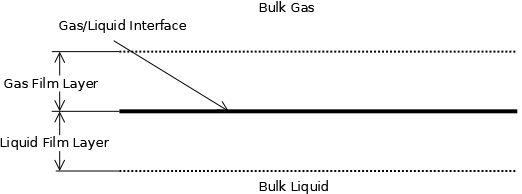
\includegraphics[width=\textwidth,height=\textheight,keepaspectratio]{GFX/twoFilm.png} 
\caption{Illustration of two film theory}
\label{twoFilm}
\end{figure}

The two film model is detailed by Albright. \cite[p. 604]{Albright2008}  In brief, the model partitions space into bulk liquid, liquid film, gas film, and  bulk gas layers.  Between the liquid and gas sfilm layers is a liquid/gas interface.  Each film layer is modeled by Whitman's stagnant film model wherein each film layer is of thickness $x_0$ and is assumed quiescent. [ibid. 602]  The mass transfer process is then governed by diffusion and the mass flux across the film layer is governed by Fick's first law,

\begin{equation}
    J = - D \frac{dC}{dx}, 
\end{equation}
where the diffusion coefficient is the mass diffusion coefficient for a particular solute.  The mass transfer coefficient for a given film layer is defined as,
\begin{equation}
    \label{kmDef}
    k_m = \frac{1}{R_m} = \frac{D}{x_0}.
\end{equation}

In this way, the mass transfer problem can be reduced to a series resistance problem, illustrated in figure \ref{fig:twoResist}
\label{fig:twoResist}
\begin{figure}[ht]
\begin{center}
    

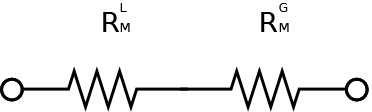
\includegraphics[width=0.5\textwidth,height=0.5\textheight,keepaspectratio]{massTwoResist.png}
\caption{Mass transfer modeled as a two resistance problem}
\end{center}
\end{figure}

According to Perry, the mass diffusion coefficients of gasses are much greater than that of liquids. \cite[sec. 5 p. 48]{Perry2008} Therefore, since ,
\begin{equation}
    D_g >> D_L,
\end{equation}
and, considering equation \ref{kmDef}, it follows,

\begin{equation}
    R_m^g+R_m^L \approx R_m^L,
\end{equation}
and the overall mass transfer coefficient, $K_m \approx 1 / R_m^L$.

We can thus approximate the mass transfer across the phase interface as,

\begin{equation}
    \label{eqn_MT_int}
    J = K_m (C^{B,L}-C^{int,L}).
\end{equation}

We next invoke Henry's law for an ideal gas which states,
\begin{equation}
    \lim_{C\to 0 }  \frac{C ^L}{p^G} = H_i.
\end{equation}
More information on Henry's law is given by Albright. \cite[p. 13]{Albright2008} Equation \ref{eqn_MT_int} can be rewritten as,

\begin{equation}
    J = K_m (C^B-H_i p_i^{F,G}).
\end{equation}
Further, we assume,
\begin{equation}
    p_i^{F,G} \approx p_i^{B,G},
\end{equation}
the partial pressure of the dissolved gas in the gas film layer is approximately equal to the partial pressure of the gas in the bulk; this is justified on the grounds that the diffusion process in gasses is much faster than the diffusion processes in liquid, consider the relative magnitudes of their mass diffusion coefficients.  Thus,

\begin{equation}
    J = K_m (C^B-H_i p_i^{B,G}).
\end{equation}

Invoking the ideal gas law, $p = CRT$, we write

\begin{equation}
    J = K_m (C^{B,L}-H RT C^{B,G}).
\end{equation}

Forms of this equation are ubiquitous in MSR xenon analysis literature.  In the transfer of mass from fuel salt to graphite, the concentration term for the graphite is divided by an effective void fraction term,

\begin{equation}
    J = K_m (C^{B,L}-\frac{H RT}\epsilon{} C^{B,G}),
\end{equation}
so the porosity of the material is accounted for.
\subsection{Ideal Gasses, Dillute Solutions, and Deviation Therefrom}
Fletcher reports a macroscopic discrete phase inclusion will form if the radius excedes the a embryo of dispersed phase atoms exceeds the critical radius,
\begin{equation}
    r_c = \frac{2\sigma}{\Delta G_V}.
\end{equation}\cite{Fletcher1958}
Westh and Haynes investigated the bounds of the domain of concentrations where Henry's Law is applicable,  the Henry region, in water and hexane using a number of solutes. \cite{Westh1998} Westh and Haynes were unable to determine the Henry region due to the limits of the calorimeter used; however, they were able to give a lower limit for non-Henry behavior on the order of $10^{-4}$, for hexane solvents and solutes, and $10^{-5}$, for a water solute and a number of solvents.   As previously mentioned, Grimes, Blander and Watson established solubility limits for xenon in molten salts, above which no further xenon could dissolve in their experimental apparatus. \cite{Grimes1958,Blander1959,Watson1962}

\begin{figure}[ht]
\centering
\includesvg[width=0.5\textwidth]{XenonConc.svg}
\caption{MSR Gas Concentration Map}
\label{concMap} 
\end{figure}
Given these observations, we posit the following: Consider figure \ref{concMap}.  This figure represents the phase space of xenon and other-gas concentrations within the molten salt system.  There is then, three regions, H,N,and B.  The Henry region, H, is where Henry's law is applicable; The Non-Henery region, N is where Henry's law is not applicable, but the salt melt has yet to reach gas saturation; finally, B, the bubble-out region, is where the salt melt has reached saturation and additional gas evolution forms dispersed gas-phase inclusions rather than dissolving into the salt melt.  No evidence has been found that indicates the H/N boundary exhibits any sort of sharp discontinuous behavior, and we suspect the transition from Henry-like to non-Henry-like behavior exhibits a \textit{smooth} character.  One potential criterion for the H/N boundary is the xenon concentration such that the ratio of the xenon to partial pressure is greater than multiple, K, of the Henry constant,
\begin{equation}
    C_i^L \; S.T. \; \frac{C_i^L}{p_i^g} > KH_i.
\end{equation}
Since the Henry constant is a function of temperature, pressure, and composition, it likewise follows the location of the  H/N boundary is a function of temperature, pressure, and composition. 
Consider a volume of salt melt with xenon and other gasses dissolved in it. This salt melt also contains actinides that are undergoing fission.  As the actinides undergo fission, a fraction of their fission products are gaseous.  If we track the behavior of these gaseous fission products, including xenon, then there is a certain probability per unit time that the gaseous products will join a gas embryo of radius greater than the critical radius.  This probability is a function of the quantity of gas within the salt melt.  We posit the N/B boundary is the total gas concentration such that a gas atom is more likely than not to join a gas embryo of radius greater than critical radius.  Since the critical radius is a function of the surface tension and Gibbs free energy, and these are functions of temperature and composition, and for the case of the Gibbs free energy, the pressure, the N/B boundary is likewise a function of temperature, pressure and composition.

All the xenon modeling efforts to date have focused on modeling efforts within the H region.  No work was found that did not use Henry's law the formulation of the mass transfer equations.
\subsection{Diffusion}
There are two diffusion coefficients used in the formulation of MSR xenon theory, one for diffusion within the graphite, and another for diffusion within the fuel-salt. 

The diffusion coefficient in the graphite is a function of the atomic mass of the diffusing species; ORNL-4069 states two different graphite mass diffusion coefficients were used in their calculations, one for Xenon and one for Krypton. \cite[p. 65]{ORNL4069} The porous media mass diffusion coefficient  encapsulates a number of mechanistically different diffusion phenomena such as viscous diffusion, Knudsen diffusion, surface diffusion, and molecular sieving. \cite[p. 190]{Cussler07}  The Knudsen mechanism was the dominate mechanism of diffusion in MSRE graphite. \cite[p. 37]{ORNL4148}  The Knudsen diffusion coefficient can be predicted from the expression,
\begin{equation}
    \label{eq:knDiff}
    D_{Kn} = \frac{L_{Pore}}{3} \left( \frac{2K_B  T}{m} \right)^{1/2}.\;  \text{\cite[p.194]{Cussler07}}
\end{equation} 
ORNL-4389 states after impregnation, the primary peak of the MSRE graphite porosity distribution occurred at 80 nm. \cite[p. 12]{ORNL4389}  The MSRE graphite temperature was between 952 and 977 K. \cite[p. 56]{Robertson1971} Given these parameters, equation \ref{eq:knDiff} evaluates to $8.7\times10^{-7} cm^2/s$, which is within the range of mass diffusion coefficients,  $3.0\times10^{-8} $ to $8.7\times10^{-5} cm^2/s$ considered feasible in the MSRE. \cite[p. 54]{ORNLTM3464}

The mass diffusion coefficient for xenon in liquid fuel-salt is used in the calculation of mass-transfer coefficients through the Sherwood number,
\begin{equation}
    Sh = \frac{k_m L}{D},
\end{equation}
which is given from mass transfer correlations of the form,
\begin{equation}
    Sh = f(Re,Sc) \text{\cite[p. 257]{Cussler07}}
\end{equation}
ORNL-4069 sates the mass diffusion coefficient can be found through analogy to a heavy-metal, water system; however, the way in which this is done was cited as a personal communication to C. Chester. \cite[p p.62]{ORNL4069} Details about the use of a water analog in a molten metal system were found in a paper by Kang et al. \cite[p. 107]{Muruganant2017} 

In addition to the heavy-metal, water analog, ORNL-4069 state the mass diffusion coefficient may be found through the Wilk-Chang equation and Stokes-Einstien equation. \cite[p. 62]{ORNL4069}
The Einstien Stokes equation,
\begin{equation}
    D = \frac{K_B T}{6 \pi \mu r_{Xe} },
\end{equation}
requires three parameters, the temperature, the viscosity, and the Atomic radii. \cite[p. 127]{Cussler07}    Viscosity data can be found in the sources by Cantor, Janz and Sohal as described in section \ref{sec:fuelSaltProperties}.\cite{ORNLTM2316,Sohal2010,Janz2013} We are unsure about what atomic radii data would be best suited for calculations.The Einstien-Stoke equation is derived assuming the diffusing particle is a hard sphere. Pau, Berg, and McMillan state, in the context of Stokes law,
\begin{quote}
    "One of the most difficult questions involved in the transition from a continuum medium to the case of real solvent molecules of size comparable to the atomic dimensions of the mobile ion is unit is the meaning to be attached to the particle 'radius'". \cite{Pau90}
\end{quote}

Several potential atomic radii are listed in table \ref{tbl:radius}. 

\ctable[caption = {Atomic Radii of Xenon},label={tbl:radius}]{lll}
{
  % You specify table footnotes here.
  \tnote[*]{Born states this value was calculated using the methods of kinetic theory outlined in his book, however, we were unable to discern precisely how this was done.}
}
{

    \FL % FLORIDA (just kidding, means "first line")
\textbf{Tpe} & \textbf{Radius [Å]} & \textbf{Reference}
\ML % middle line
Covalent Radius                 &   1.36     &\cite[p. 9-58]{CRCChemPhy97}   \\ 
van der Waal's Radius           &   2.16     &[ibid.]                        \\ 
Lennard-Jones Collision Radius  &   2.02     &\cite[p.24]{R132}              \\
Kinetic Theory*                 &   1.75     &\cite[p. 249]{Born13}         \\
\LL % last line
}

Given the radiation field present in an MSR, 

An additional complexity arises in considering the effect xenon ionization has on the atomic radius.  Born states,

\begin{quote}
    "We see\footnote{in an attached tabulation of ionic radii } that the negative ions, which have an inert gas configuration with a smaller nuclear charge then the corresponding inert gas, are larger than the latter, the reason being of course tha the electrons in these ions are more loosely bound so that their orbits have greater radii.  A corresponding, mutatis mutandis, hold for positive ions also."
\end{quote}
Thus, the ionic radius is a function of the degree of ionization of the xenon. 

According to James, the average kinetic energy of fission fragments is in excess of 160 MeV. \cite{James69} Oberstedt, Bilnert, and Gatera state the prompt gamma ray energy from U-235 fission is in excess of 6 MeV.\cite[p. 86]{Oberstedt15}  In addition to these sources of energy, we assert there exists radiation, in the form of alpha, beta, and gamma emanation, from the fission fragments. The sum of all the ionization energies in xenon is ~0.2 MeV. \cite{NIST_XE}  It therefore follows the radiation field in an MSR is capable of completely ionizing any xenon in the reactor.

Since the ionic radius is a function of the degree of ionization, and the xenon in a MSR may be ionized, it follows that any consideration into atomic radius ought to consider the effect of ionization on the atomic radius.  A corollary to this is the data in talbe \ref{tbl:radius} may be greater than the effective atomic radius of xenon an in MSR.  Furthermore, since,
\begin{equation}
    Sh \propto \frac{1}{D} \wedge D \propto \frac{1}{r_{Xe}} \implies Sh \propto r_{Xe} \implies k_m \propto r_{Xe},
\end{equation}
it follows that the mass transfer coefficients, $k_m$, in a nuclear system will be lower than those in a non-nuclear mockup. 

liquid: ways to do it on p.62



\section{TODO}
The potential for parameterization/operationalization/generalization catastrophe
Geometric index, biot number, and irregular shapes.

TODO: MORE ABOUT THE STATE.
\printbibliography

\end{document}


